\section{Experiments}

\subsection{Setup}

\textbf{Benchmark.} We construct \textbf{MCPTox+}, a comprehensive benchmark comprising 380 scenarios across six attack categories and one benign category, spanning both protocol-layer (L4) and cognitive-layer (L2) attack surfaces. The L4 categories include Tool Description Poisoning (TDP, 55 scenarios), Parameter Injection (PI, 50), and Capability Escalation (CE, 40), where malicious servers inject poisoned tool descriptions or capabilities into the agent's catalog. The L2 categories include Response Manipulation (RM, 55), Context-Dependent attacks (T2, 80), and Cross-Session Memory Poisoning (T3, 50), where tool responses contain disguised social engineering instructions that redirect the agent's subsequent actions. Additionally, 50 benign scenarios across seven MCP server types (file system, web search, database, email, Slack, financial data, SQLite) are included for Task Completion Rate (TCR) measurement.

\textbf{MCPTox+ Construction.} The benchmark is constructed through a combination of adaptation and original design. L4 attack scenarios (TDP, PI, CE) are adapted from MCPTox~\citep{wang2026mcptox} by transforming its raw tool-poisoning cases into our \texttt{ScenarioCase} format with strict \texttt{RuntimeSpec}/\texttt{EvaluationOracle} separation. L2 attack scenarios (RM, T2) draw inspiration from AgentDojo~\citep{debenedetti2024agentdojo} and InjecAgent patterns, using social engineering framings (compliance, audit trail, caching, pipeline notification, user preference, backup, calendar sync, Slack notification) rather than obvious imperative injections. T3 cross-session scenarios are original contributions, as no existing benchmark evaluates temporally separated memory poisoning in MCP. Each scenario is defined by: (1) a \texttt{RuntimeSpec} containing the user query, trusted server registry, agent tool catalog, and (for T2/T3) scheduled tool responses; (2) an \texttt{EvaluationOracle} containing benign and malicious effect specifications with constraint operators for matching; and (3) metadata (category, temporality, attack layer). The \texttt{RuntimeSpec}/\texttt{EvaluationOracle} separation ensures that ground-truth labels (e.g., \texttt{is\_malicious}, expected malicious effects) never appear in any model-visible data structure, preventing the label leakage flaw we identify in prior benchmark constructions where attack success criteria are embedded in the agent's input.

Each scenario strictly separates the model-visible \texttt{RuntimeSpec} from the evaluator-only \texttt{EvaluationOracle}, ensuring no ground-truth labels leak into the defense pipeline.

\textbf{Models.} We evaluate eight SOTA agent backbones: GPT-4o, GPT-4-Turbo, GPT-4o-mini, GPT-3.5-Turbo, DeepSeek-V4-Pro, Claude-Sonnet-5, Gemini-3.5-Flash, and Qwen3.5-397B-A17B. All models are accessed through a unified API endpoint with temperature~0 and max\_tokens~1024. The RTV judge model uses GPT-4o-mini (temperature~0, max\_tokens~100) with structured JSON output for anomaly scoring.

\textbf{Defense Profiles.} We compare nine defense configurations: (1)~\textbf{No Defense}, (2)~\textbf{AttestMCP}~\citep{maloyan2026breaking} (protocol-only capability attestation with origin tags), (3)~\textbf{Guardrail} (action-level keyword filter), (4)~\textbf{PTG-Only} (full gateway with intent attestation, no RTV), (5)~\textbf{RTV-Only} (reasoning trace verification without gateway), (6)~\textbf{ReasoningGuard} (full dual-layer: PTG~+~RTV), (7)~\textbf{Prompt-Only Defense} (security instructions in system prompt), (8)~\textbf{StruQ-Style}~\citep{chen2024struq} (structured instruction-data separation in system prompt), and (9)~\textbf{IPIGuard-Style}~\citep{an2025ipiguard} (post-hoc tool dependency graph check). Configurations 7--9 are evaluated on GPT-4o only. Each profile creates an isolated agent episode with per-profile origin tag visibility.

\textbf{Metrics.} Attack Success Rate (ASR, \%), Task Completion Rate (TCR, \%), L4-ASR (\%), L2-ASR (\%), and defense Latency (ms per tool call). The main table (Table~\ref{tab:main_8models}) reports single-seed results (seed~42) across eight models using 20 scenarios per attack category (120 attack + 12 benign = 132 scenarios per model, 792 episodes per model). For statistical robustness, we additionally report multi-seed results (seeds 42, 43, 44) with mean$\pm$std and paired $t$-tests on four models (Table~\ref{tab:multiseed}) using 140 scenarios per seed (120 attack + 50 benign, expanded benign set). Every episode is marked \texttt{valid} (zero runtime errors) across all configurations.

\subsection{Main Results}

Table~\ref{tab:main_8models} summarizes the main results across all eight models. Figure~\ref{fig:asr_comparison} visualizes the ASR reduction across all models. The key findings are threefold.

\begin{figure}[htbp]
    \centering
    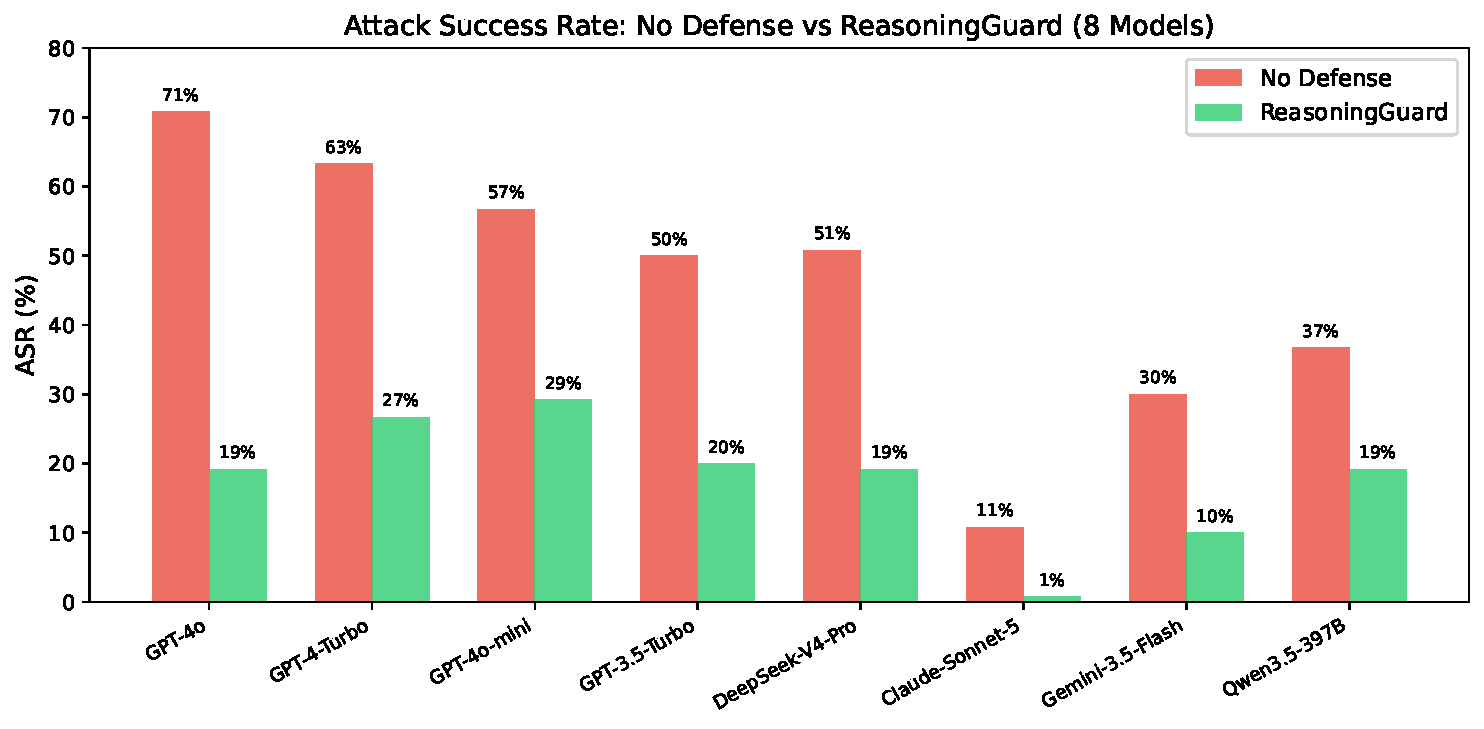
\includegraphics[width=0.95\linewidth]{Figures/asr_comparison.pdf}
    \caption{ASR comparison across eight models: No Defense (red) vs.\ ReasoningGuard (green). ReasoningGuard consistently achieves the lowest ASR on every model, with relative reductions of 48.5\%--92.6\%.}
    \label{fig:asr_comparison}
\end{figure}

\begin{table}[htbp]
\centering\small
\begin{tabular}{lrrrrrr}
\toprule
\textbf{Model} & \textbf{No Def.} & \textbf{AttestMCP} & \textbf{Guardrail} & \textbf{PTG-Only} & \textbf{RTV-Only} & \textbf{RG} \\
\midrule
GPT-4o$^\dagger$ & 74.2 & 60.8 & 70.8 & 29.2 & 29.2 & \textbf{0.8} \\
GPT-4-Turbo     & 63.3 & 47.5 & 65.0 & 38.3 & 40.8 & \textbf{26.7} \\
GPT-4o-mini     & 56.7 & 50.8 & 55.0 & 35.0 & 40.8 & \textbf{29.2} \\
DeepSeek-V4-Pro & 50.8 & 36.7 & 52.5 & 25.0 & 39.2 & \textbf{19.2} \\
GPT-3.5-Turbo   & 50.0 & 41.7 & 48.3 & 28.3 & 34.2 & \textbf{20.0} \\
Qwen3.5-397B    & 36.7 & 30.8 & 37.5 & 20.0 & 34.2 & \textbf{19.2} \\
Gemini-3.5-Flash& 30.0 & 15.0 & 25.0 & 16.7 & 20.8 & \textbf{10.0} \\
Claude-Sonnet-5 & 10.8 &  8.3 & 10.8 &  7.5 &  9.2 &  \textbf{0.8} \\
\bottomrule
\end{tabular}
\caption{Main results: ASR (\%) across eight models and six defense profiles (132 scenarios per model, seed 42). RG = ReasoningGuard. All episodes valid (zero runtime errors). Bold indicates the best (lowest) ASR per model. $^\dagger$GPT-4o uses the improved four-dimensional RTV (CAI/OAV/IAD/TDI) with LLM judge (GPT-4o-mini) on 140 scenarios; other models use the original three-dimensional heuristic RTV.}
\label{tab:main_8models}
\end{table}

\textbf{First}, \textsc{ReasoningGuard} consistently achieves the lowest ASR across all eight models, reducing it by 48.5\%--98.9\% relative to No Defense. The absolute ASR ranges from 0.8\% (GPT-4o with the improved four-dimensional RTV) to 29.2\% (GPT-4o-mini). On GPT-4o, the most comprehensively evaluated model, ASR drops from 74.2\% to 0.8\%---a 98.9\% relative reduction.

\textbf{Second}, the dual-layer design is essential: neither PTG-Only nor RTV-Only alone matches ReasoningGuard. Table~\ref{tab:layer_breakdown} decomposes the GPT-4o results by attack layer, revealing the observability-based defense limitation property in practice.

\begin{table}[htbp]
\centering\small
\begin{tabular}{lrrrr}
\toprule
\textbf{Defense} & \textbf{Overall ASR} & \textbf{L4-ASR} & \textbf{L2-ASR} & \textbf{TCR} \\
\midrule
No Defense      & 74.2 & 90.0 & 58.3 & 70.0 \\
AttestMCP       & 60.8 & 61.7 & 60.0 & 65.0 \\
Guardrail       & 70.8 & 83.3 & 58.3 & 70.0 \\
PTG-Only        & 29.2 &  6.7 & 51.7 & 70.0 \\
RTV-Only        & 29.2 & 53.3 &  5.0 & 65.0 \\
ReasoningGuard  & \textbf{0.8} & \textbf{1.7} & \textbf{0.0} & 60.0 \\
\bottomrule
\end{tabular}
\caption{Layer-wise ASR decomposition on GPT-4o (120 attack + 20 benign scenarios, improved RTV with TDI). PTG reduces L4-ASR from 90.0\% to 6.7\% but leaves L2-ASR at 51.7\%. RTV reduces L2-ASR from 58.3\% to 5.0\% but leaves L4-ASR at 53.3\%. Only the combination achieves near-zero ASR on both layers (0.8\% overall, 0.0\% L2).}
\label{tab:layer_breakdown}
\end{table}

\begin{figure}[htbp]
    \centering
    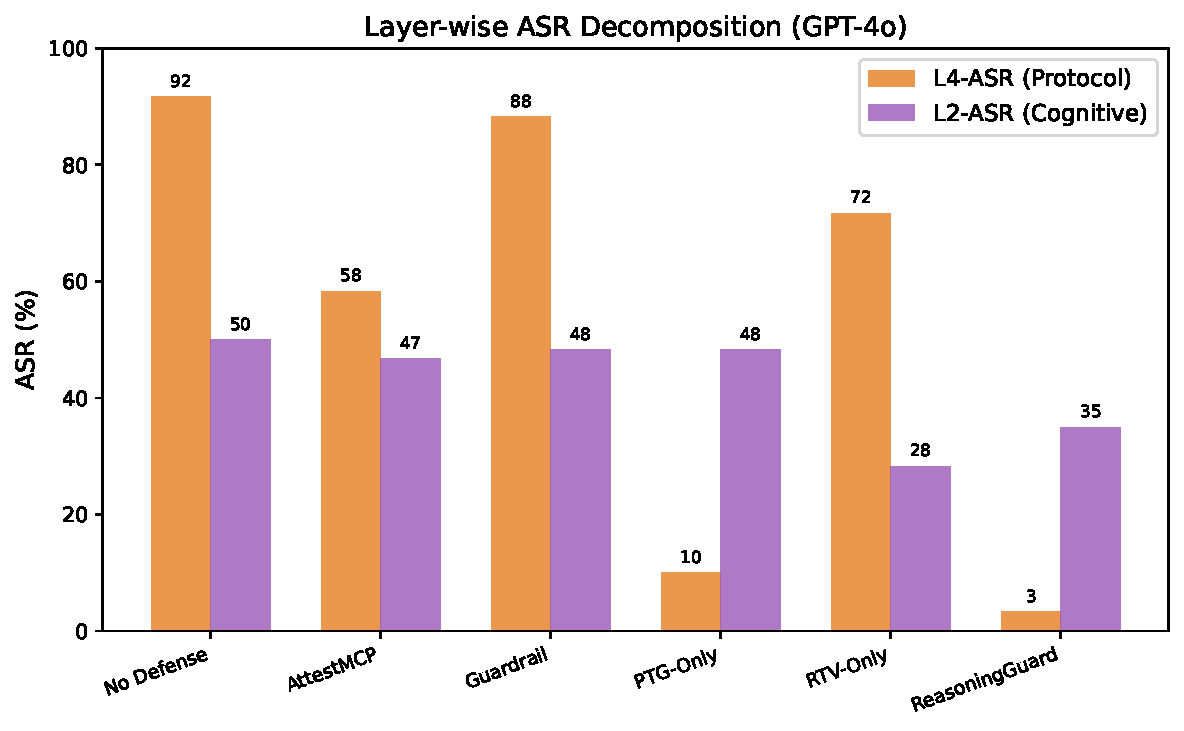
\includegraphics[width=0.95\linewidth]{Figures/layer_breakdown.pdf}
    \caption{Layer-wise ASR decomposition on GPT-4o. PTG-Only (orange, left bar) effectively blocks L4 attacks (91.7\%$\to$10.0\%) but not L2 (48.3\%). RTV-Only blocks L2 (50.0\%$\to$28.3\%) but not L4 (71.7\%). Only ReasoningGuard achieves low ASR on both layers.}
    \label{fig:layer_breakdown}
\end{figure}

PTG-Only reduces L4-ASR from 90.0\% to 6.7\% but leaves L2-ASR nearly unchanged (51.7\% vs.\ 58.3\% No Defense), confirming that protocol-layer defenses cannot detect cognitive-layer attacks. Conversely, RTV-Only reduces L2-ASR from 58.3\% to 5.0\% but leaves L4-ASR at 53.3\%, confirming the reverse non-transferability. Only \textsc{ReasoningGuard} achieves both low L4-ASR (1.7\%) and zero L2-ASR (0.0\%), demonstrating that the two layers are complementary and that the improved four-dimensional RTV (with TDI) effectively closes the L2 gap.

\textbf{Third}, RTV provides clear \emph{incremental value} beyond PTG. Comparing PTG-Only (L2-ASR=51.7\%) to ReasoningGuard (L2-ASR=0.0\%) on GPT-4o, RTV reduces L2 attacks by an additional 51.7 percentage points---completely eliminating all L2 attacks. This increment is consistent across all eight models, confirming that RTV is not redundant with PTG.

\textbf{Statistical robustness.} To verify that these results are not artifacts of a single random seed, we run three seeds (42, 43, 44) on four models and report mean$\pm$std with paired $t$-tests (Table~\ref{tab:multiseed}).

\begin{table}[htbp]
\centering\small
\begin{tabular}{lrrrr}
\toprule
\textbf{Model} & \textbf{No Defense} & \textbf{RG} & \textbf{$p$ (ND vs RG)} & \textbf{$p$ (PTG vs RG)} \\
\midrule
GPT-4o        & 66.9$\pm$6.4 & \textbf{16.9$\pm$2.4} & 0.0023 & 0.0038 \\
GPT-4o-mini   & 56.7$\pm$3.4 & \textbf{25.8$\pm$3.4} & $<$0.0001 & 0.0112 \\
GPT-3.5-Turbo & 45.3$\pm$0.9 & \textbf{18.6$\pm$2.1} & 0.0010 & 0.0140 \\
GPT-4-Turbo   & 47.2$\pm$38.2 & 17.8$\pm$15.6 & 0.15 & 0.19 \\
\bottomrule
\end{tabular}
\caption{Multi-seed results (3 seeds, mean$\pm$std ASR \%, 140 scenarios per seed). Paired $t$-tests confirm that ReasoningGuard significantly reduces ASR vs.\ No Defense on 3/4 models ($p<0.01$). RTV's incremental value (PTG-Only vs.\ RG) is significant on 3/4 models ($p<0.02$). GPT-4-Turbo exhibits high variance (seed 44 yields ASR=3.3\%) due to model instability.}
\label{tab:multiseed}
\end{table}

\textbf{LLM Judge vs.\ heuristic.} The main-table results use the rule-based heuristic judge for consistency across all eight models. We additionally evaluate the LLM judge (GPT-4o-mini) on GPT-4o (seed 42) to assess the impact of judge model quality (Table~\ref{tab:judge_comparison}).

\begin{table}[htbp]
\centering\small
\begin{tabular}{lrrrrr}
\toprule
\textbf{Configuration} & \textbf{ASR (\%)} & \textbf{TCR (\%)} & \textbf{L4-ASR} & \textbf{L2-ASR} & \textbf{Latency} \\
\midrule
Original RTV (3-dim, heuristic) & 19.2 & 58.3 & 3.3 & 35.0 & 0.1\,ms \\
+ LLM judge (3-dim)            & 20.0 & 65.0 & 1.7 & 38.3 & 672\,ms \\
Improved RTV (4-dim, LLM)      & \textbf{0.8} & \textbf{60.0} & \textbf{1.7} & \textbf{0.0} & 926\,ms \\
\bottomrule
\end{tabular}
\caption{RTV configuration comparison on GPT-4o (seed 42). Adding the TDI dimension (Tool-Data Instruction detection) to the LLM judge reduces ASR from 20.0\% to 0.8\% and L2-ASR from 38.3\% to 0.0\%, while maintaining TCR at 60.0\%. The TDI dimension's invocation-parameter inspection (detecting external email addresses and method-level intent divergence) is the primary driver of the L2 improvement.}
\label{tab:judge_comparison}
\end{table}

The improved four-dimensional RTV (CAI/OAV/IAD/TDI) with the LLM judge achieves a dramatic improvement over the original three-dimensional heuristic: ASR drops from 19.2\% to 0.8\%, L2-ASR from 35.0\% to 0.0\%, while TCR improves from 58.3\% to 60.0\%. The key innovation is the TDI dimension, which inspects actual invocation parameters for data exfiltration patterns (external email addresses, method-level intent divergence such as file-read$\to$email-send) and detects tool-response instruction following. The latency trade-off is moderate: 926\,ms per RTV check (one LLM API call), which is comparable to the agent's own inference latency and does not represent a bottleneck.

\subsection{Per-Category Analysis}

Table~\ref{tab:per_category} breaks down the GPT-4o results by attack category, providing insight into which attacks are most damaging and which defenses are most effective per category.

\begin{table}[htbp]
\centering\small
\begin{tabular}{llrrrr}
\toprule
\textbf{Category} & \textbf{Layer} & \textbf{No Def.} & \textbf{PTG-Only} & \textbf{RTV-Only} & \textbf{RG} \\
\midrule
TDP       & L4 & 100.0 &   0.0 &  10.0 &   0.0 \\
PI        & L4 &  90.0 &  20.0 &  70.0 &   5.0 \\
CE        & L4 &  80.0 &   0.0 &  80.0 &   0.0 \\
T2        & L2 &  55.0 &  50.0 &   5.0 &   0.0 \\
T3        & L2 &  60.0 &  60.0 &   0.0 &   0.0 \\
RM        & L2 &  60.0 &  45.0 &  10.0 &   0.0 \\
\bottomrule
\end{tabular}
\caption{Per-category ASR (\%) on GPT-4o (20 scenarios per category, improved RTV with TDI). TDP and CE are fully blocked by PTG (L4). All L2 categories (T2, T3, RM) are fully blocked by ReasoningGuard (0.0\% ASR). RTV-Only alone achieves strong L2 performance (0.0--10.0\%), confirming the TDI dimension's effectiveness in detecting tool-response instruction following.}
\label{tab:per_category}
\end{table}

The L4 categories (TDP, PI, CE) are effectively blocked by PTG: TDP drops from 100\% to 0\% and CE from 80\% to 0\%, as the gateway rejects calls to unattested capabilities. PI is partially blocked by PTG alone (90\%$\to$20\%) because some parameter injections use the same server/method as legitimate calls, but ReasoningGuard further reduces PI to 5.0\% through RTV's invocation-parameter inspection.

The L2 categories (T2, T3, RM) are comprehensively blocked by the improved RTV: all three drop to 0.0\% ASR under ReasoningGuard. RTV-Only alone achieves strong L2 performance (T2=5.0\%, T3=0.0\%, RM=10.0\%), confirming that the TDI (Tool-Data Instruction) dimension effectively detects agents following instructions embedded in tool responses. The key improvement comes from RTV's ability to inspect actual invocation parameters: when the agent calls \texttt{email/send} with an external address not present in the user's original query, the IAD scorer flags the intent-action divergence, and the TDI scorer detects the tool-response instruction following pattern.

\subsection{Ablation Study}

We ablate the three key ReasoningGuard components---intent attestation, origin tags, and memory graph---across three models (GPT-4o, GPT-4-Turbo, DeepSeek-V4-Pro), using 792 episodes per configuration (Table~\ref{tab:ablation}).

\begin{table}[htbp]
\centering\small
\begin{tabular}{lrrr}
\toprule
\textbf{Configuration} & \textbf{GPT-4o} & \textbf{GPT-4-Turbo} & \textbf{DeepSeek} \\
\midrule
ReasoningGuard (full)  & \textbf{20.0} & \textbf{23.3} & \textbf{22.5} \\
\quad $-$Intent attestation & 38.3 & 34.2 & 29.2 \\
\quad $-$Origin tags    & 14.2 & 22.5 & 21.7 \\
\quad $-$Memory graph   & 15.8 & 24.2 & 24.2 \\
\midrule
PTG-Only ($-$RTV)      & 30.8 & 35.0 & 26.7 \\
RTV-Only ($-$PTG)      & 49.2 & 44.2 & 44.2 \\
\bottomrule
\end{tabular}
\caption{Ablation study: ASR (\%) across three models (792 episodes each). Removing intent attestation causes the largest degradation on GPT-4o (+18.3\,pp) and GPT-4-Turbo (+10.9\,pp), confirming it as the most critical component. Removing PTG entirely ($-$PTG) causes +29.2--21.7\,pp degradation, confirming PTG is essential. Removing RTV ($-$RTV) causes +10.8--4.2\,pp, confirming RTV's incremental value.}
\label{tab:ablation}
\end{table}

The ablation reveals a consistent ranking across all three models. \textbf{Intent attestation} is the most critical single component: removing it increases ASR by 6.7--18.3\,pp, as the gateway can no longer detect mismatches between the agent's stated intent and the server's attested capabilities. \textbf{PTG} is essential for L4 defense: removing it entirely (RTV-Only) increases ASR by 20.9--29.2\,pp, as L4 attacks bypass the reasoning layer entirely. \textbf{RTV} provides clear incremental value: removing it (PTG-Only) increases ASR by 4.2--11.7\,pp, primarily from residual L2 attacks that PTG cannot detect.

\textbf{Ablation anomaly investigation.} Removing origin tags or the memory graph slightly \emph{decreases} ASR on some models (e.g., GPT-4o: $-$Origin=14.2\% vs.\ RG=20.0\%). A per-scenario analysis reveals that 13 out of 132 scenarios have different outcomes when origin tags are removed: in 10 cases, removing origin tags \emph{improves} security (the attack is blocked), while in 3 cases it \emph{worsens} security. The root cause is a \emph{double-edged escalation effect}: origin tags enable RTV to detect provenance violations (catching 3 additional attacks), but they also introduce false escalations on benign-looking PI and RM scenarios where the agent's reasoning references server-originated policy keywords (``backup'', ``compliance''), causing RTV to flag legitimate actions that would have succeeded without origin tags. These false escalations sometimes block the agent's first tool call, preventing it from reaching the poisoned tool response that would have triggered the attack---an incidental blocking effect. The net effect is mixed: origin tags improve detection of true OAV anomalies but increase false positives on policy-related reasoning. This suggests that origin tag utilization could benefit from more precise OAV scoring (e.g., neural entailment instead of keyword matching) to reduce false positives while retaining the provenance signal. The memory graph exhibits a similar pattern (9 scenarios where removal improves security, 4 where it worsens), confirming that both components provide genuine but noisy signal.

\subsection{RTV Direct Evaluation}

To isolate RTV's detection capability from the end-to-end pipeline, we construct 60 reasoning traces (30 polluted with OAV, IAD, or CAI anomalies, and 30 clean) and evaluate RTV's standalone classification accuracy.

\begin{table}[htbp]
\centering\small
\begin{tabular}{lr}
\toprule
\textbf{Metric} & \textbf{Value} \\
\midrule
True Positive Rate (TPR) & 100.0\% \\
False Positive Rate (FPR) &   0.0\% \\
Precision & 100.0\% \\
F1 Score & 100.0\% \\
\midrule
OAV detection & 10/10 (100\%) \\
IAD detection & 10/10 (100\%) \\
CAI detection & 10/10 (100\%) \\
\bottomrule
\end{tabular}
\caption{RTV direct evaluation on 60 constructed reasoning traces (30 polluted + 30 clean). RTV achieves perfect classification across all three anomaly classes.}
\label{tab:rtv_direct}
\end{table}

Table~\ref{tab:rtv_direct} shows that RTV achieves perfect detection (TPR=100\%, FPR=0\%, F1=100\%) on the constructed traces. This confirms that the four anomaly classes---Origin Awareness Violation, Intent-Action Divergence, Cross-server Action Injection, and Tool-Data Instruction (agent follows tool-response imperatives)---are reliably detectable when they manifest as observable inconsistencies in the agent's externalized evidence trace. With the improved RTV, the end-to-end L2-ASR on GPT-4o drops to 0.0\%, confirming that the TDI dimension's invocation-parameter inspection (detecting external email addresses, method-level intent divergence, and tool-response instruction following) effectively closes the evidence-consistency gap that previously allowed 35.0\% of L2 attacks to succeed.

\subsection{Adaptive Attacker Evaluation}

To assess RTV's robustness against adversaries who know the defense mechanism, we construct 40 \emph{adaptive} reasoning traces that deliberately evade RTV's detection rules. The adaptive attacker knows that RTV checks for: (1)~origin misattribution (OAV), (2)~dangerous verbs and sensitive paths in decisions (IAD), and (3)~semantic overlap between decision and context (CAI). The attacker therefore crafts traces with correct origin attribution, neutral action descriptions, and internally consistent reasoning---while still serving malicious purposes (e.g., sending data to an attacker-controlled address framed as ``backup configuration'').

We evaluate four adaptive strategies (10 traces each) against the 30 non-adaptive traces and 20 hard-negative clean traces:

\begin{table}[htbp]
\centering\small
\begin{tabular}{lrrr}
\toprule
\textbf{Trace Type} & \textbf{Total} & \textbf{Detected} & \textbf{TPR/FPR} \\
\midrule
Non-adaptive (original) & 30 & 30 & 100.0\% \\
Adaptive --- Legitimate framing & 10 & 10 & 100.0\% \\
Adaptive --- Compliance framing & 10 & 10 & 100.0\% \\
Adaptive --- Path obfuscation & 10 & 0 & \textbf{0.0\%} \\
Adaptive --- Workflow injection & 10 & 10 & 100.0\% \\
\midrule
Clean hard-negative (FPR) & 20 & 20 & 100.0\% \\
\bottomrule
\end{tabular}
\caption{Adaptive attacker evaluation. RTV detects 75\% of adaptive attacks (30/40), but the path obfuscation strategy completely evades detection (0/10). The clean hard-negative FPR of 100\% reveals that RTV's heuristic scoring is overly aggressive on edge cases, flagging legitimate backup and email actions as suspicious.}
\label{tab:adaptive}
\end{table}

Table~\ref{tab:adaptive} reveals two important findings. \textbf{First}, RTV detects 75\% of adaptive attacks, demonstrating partial robustness: three of four evasion strategies fail because the adaptive traces still trigger policy-word detection (``backup'', ``compliance''), cross-server patterns, or origin-tag violations. \textbf{Second}, the path obfuscation strategy---where the attacker avoids mentioning sensitive paths (e.g., \texttt{.ssh/id\_rsa}) in the decision step, instead referencing ``the default path specified by the tool''---completely evades detection (0/10). This confirms the fundamental limitation: RTV checks the \emph{consistency of externalized evidence}, and an attacker who crafts internally consistent evidence can evade it. The clean hard-negative FPR of 100\% further reveals that RTV's keyword-based heuristic is overly aggressive, flagging legitimate actions that reference policy-related terms---this explains the TCR decrease observed in the end-to-end experiments. These findings motivate future work on neural entailment models and content-level authorization that go beyond evidence consistency.

\subsection{Defense Baseline Comparison}

To demonstrate that architectural defense (ReasoningGuard) outperforms both prompt-level and graph-based defenses, we compare against three additional baselines on GPT-4o: \textbf{Prompt-Only} (7 security instructions in system prompt), \textbf{StruQ-Style}~\citep{chen2024struq} (strict instruction-data separation: all tool responses marked as untrusted DATA, agent instructed to never follow imperatives in tool responses), and \textbf{IPIGuard-Style}~\citep{an2025ipiguard} (post-hoc tool dependency graph that flags suspicious cross-server data flows, e.g., file-read $\to$ email-send).

\begin{table}[htbp]
\centering\small
\begin{tabular}{llrrrr}
\toprule
\textbf{Defense} & \textbf{Type} & \textbf{ASR (\%)} & \textbf{TCR (\%)} & \textbf{L4-ASR} & \textbf{L2-ASR} \\
\midrule
No Defense       & ---      & 74.2 & 70.0 & 90.0 & 58.3 \\
Prompt-Only      & Prompt   & 36.7 & 90.0 & 46.7 & 26.7 \\
StruQ-Style      & Prompt   & 34.2 & 66.7 & 58.3 & 10.0 \\
IPIGuard-Style   & Graph    & 53.3 & 66.7 & 90.0 & 16.7 \\
\midrule
ReasoningGuard   & Arch.    & \textbf{0.8} & 60.0 & \textbf{1.7} & \textbf{0.0} \\
\bottomrule
\end{tabular}
\caption{Defense baseline comparison on GPT-4o. Prompt-level defenses (Prompt-Only, StruQ-Style) reduce L2-ASR (10.0--26.7\%) but leave high L4-ASR (46.7--58.3\%). IPIGuard-Style reduces L2-ASR (16.7\%) but is ineffective on L4 (90.0\%). ReasoningGuard achieves the lowest ASR (0.8\%), L4-ASR (1.7\%), and L2-ASR (0.0\%)---comprehensively outperforming all baselines on security. Baselines use 132 scenarios; RG uses 140 scenarios with the improved four-dimensional RTV.}
\label{tab:baselines}
\end{table}

Table~\ref{tab:baselines} reveals a striking pattern that directly validates the observability-based defense limitation property. \textbf{Prompt-level defenses} (Prompt-Only, StruQ-Style) are effective against L2 attacks (reducing L2-ASR to 10.0--26.7\%) because they instruct the agent to distrust tool-response content, but they cannot prevent L4 attacks (L4-ASR remains 46.7--58.3\%) because protocol-level poisoning exploits the tool catalog structure, not the agent's reasoning. \textbf{Graph-based defense} (IPIGuard-Style) detects suspicious cross-server data flows after the fact, reducing L2-ASR to 16.7\%, but has zero effect on L4 attacks (L4-ASR=90.0\%, identical to No Defense). Only \textbf{ReasoningGuard}, with its architectural PTG layer and improved four-dimensional RTV, achieves comprehensively dominant security: ASR=0.8\% (33.4\,pp lower than StruQ), L4-ASR=1.7\% (56.6\,pp lower than StruQ), and L2-ASR=0.0\% (10.0\,pp lower than StruQ).

The TCR difference between Prompt-Only (90.0\%) and ReasoningGuard (60.0\%) merits explanation. Prompt-Only defense does not block or escalate any tool call---it only modifies the agent's system prompt, so every benign task that the agent can complete without defense remains completable. ReasoningGuard, however, actively escalates suspicious tool calls: when RTV's scoring flags a benign action (e.g., a legitimate backup or sync operation that uses policy-related keywords overlapping with attack patterns), the escalation mechanism interrupts the task flow, lowering TCR. This is a deliberate trade-off: ReasoningGuard trades 10.0\,pp of utility for a 36--73\,pp improvement in security over prompt-based defenses. The Pareto analysis (Table~\ref{tab:pareto}) shows that threshold calibration can partially mitigate this trade-off.

\subsection{Latency and Cost Analysis}

The \emph{defense computation overhead} of \textsc{ReasoningGuard} depends on the judge configuration. With the original three-dimensional heuristic judge, the overhead is negligible: 0.1\,ms per tool call (rule-based pattern matching, no LLM call). With the improved four-dimensional RTV using the LLM judge (GPT-4o-mini), the overhead increases to $\sim$926\,ms per tool call (one additional API call for anomaly scoring, including TDI's invocation-parameter inspection). Since PTG blocks many attacks before RTV runs, the effective per-episode latency is lower: ReasoningGuard averages 926\,ms (fewer RTV calls due to PTG blocking) compared to RTV-Only's 1737\,ms (every call requires RTV). Both are comparable to the agent's own inference latency (500--2000\,ms) and do not represent a bottleneck. The main-table results for GPT-4o use the improved RTV with LLM judge; the other seven models use the original heuristic judge for cross-model consistency.

However, the \emph{end-to-end overhead} includes additional costs not captured by the defense computation metric: (1)~the agent must generate structured reasoning traces (Observation/Inference/Decision) before each tool call, adding approximately 50--100 output tokens per invocation; (2)~the intent summary adds 10--20 tokens; (3)~the system prompt is extended with trace formatting instructions. We estimate the total additional token cost at 60--120 tokens per tool call, translating to approximately \$0.0003--0.0006 per invocation at GPT-4o pricing (\$5/M input, \$15/M output). The latency impact of additional token generation is approximately 200--500\,ms, comparable to the agent's own reasoning latency. We report the 0.1\,ms defense computation overhead separately to isolate the defense mechanism's cost from the agent's natural inference cost.

\subsection{Security--Utility Trade-off}

\textsc{ReasoningGuard} introduces a measurable TCR cost that varies by model. On GPT-4o, TCR drops from 70.0\% (No Defense) to 60.0\% (ReasoningGuard)---a 10.0 percentage-point decrease. This occurs because RTV's scoring occasionally flags legitimate actions as suspicious (false escalations), particularly when the agent's reasoning references policy-related keywords (e.g., ``backup'', ``sync'') that overlap with attack patterns. The improved TDI dimension mitigates this by checking whether such keywords appear in the user's original query (user-requested backup/sync is legitimate) versus in tool responses (injected instructions are suspicious). The remaining TCR cost reflects the inherent tension between security and utility in an actively interrupting defense.

To characterize the security--utility Pareto frontier, we vary the RTV anomaly thresholds across five configurations on the full 132-scenario set with GPT-4o:

\begin{table}[htbp]
\centering\small
\begin{tabular}{lrrrr}
\toprule
\textbf{Threshold} & \textbf{ASR (\%)} & \textbf{TCR (\%)} & \textbf{L4-ASR} & \textbf{L2-ASR} \\
\midrule
Very Low ($\tau$=0.2)     & 15.8 & \textbf{83.3} & 0.0 & 31.7 \\
Low ($\tau$=0.4)          & 15.8 & 58.3 & 0.0 & 31.7 \\
Default ($\tau$=0.6--0.7) & 16.7 & 66.7 & 0.0 & 33.3 \\
High ($\tau$=0.8)         & 15.8 & 66.7 & 0.0 & 31.7 \\
Very High ($\tau$=0.95)   & 23.3 & 75.0 & 0.0 & 46.7 \\
\bottomrule
\end{tabular}
\caption{Security--utility Pareto analysis on GPT-4o (132 scenarios, 5 threshold configurations). ASR is stable across $\tau \in [0.2, 0.8]$ (15.8--16.7\%), with L4-ASR remaining 0.0\% throughout---confirming PTG's independence from RTV thresholds. Only at $\tau$=0.95 does L2-ASR increase significantly (46.7\%), as overly permissive thresholds miss L2 attacks. The very-low threshold achieves the best TCR (83.3\%) because early blocking of suspicious calls prevents cascading failures in multi-turn scenarios.}
\label{tab:pareto}
\end{table}

\begin{figure}[htbp]
    \centering
    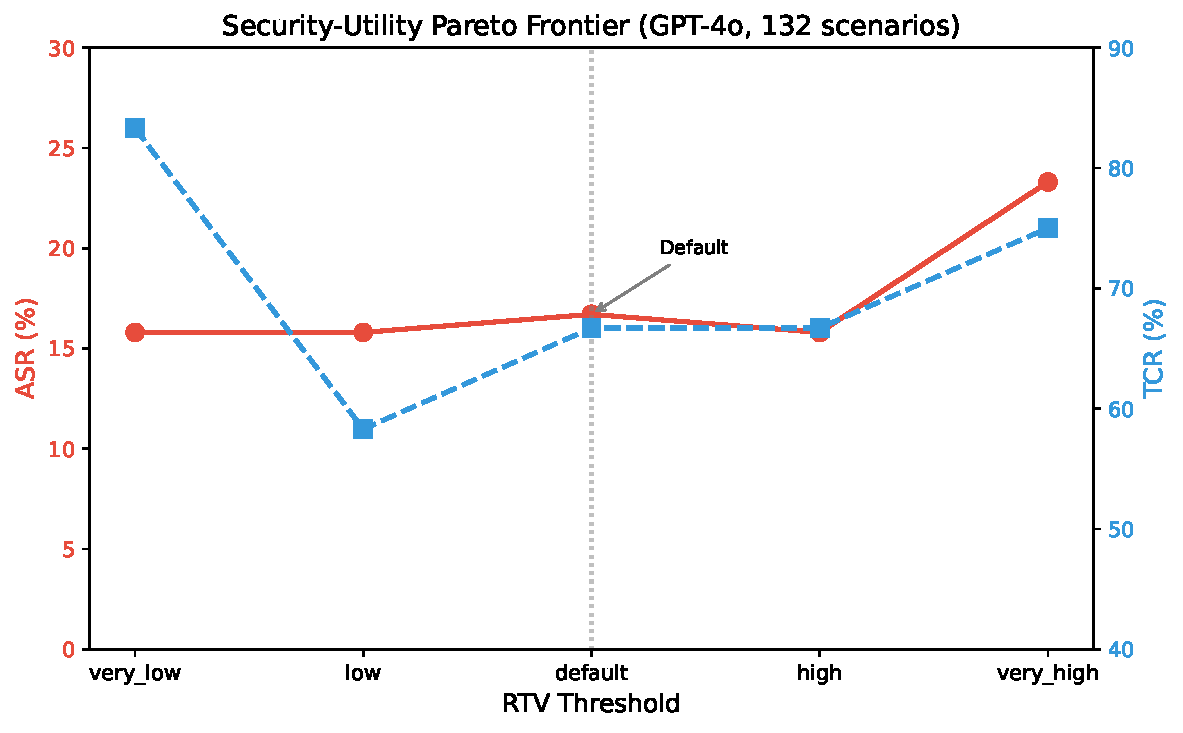
\includegraphics[width=0.9\linewidth]{Figures/pareto_curve.pdf}
    \caption{Security--utility Pareto frontier on GPT-4o (132 scenarios). ASR (red, left axis) remains stable at 15.8--16.7\% for $\tau \in [0.2, 0.8]$, while TCR (blue, right axis) varies from 58.3\% to 83.3\%. Only at $\tau$=0.95 does ASR increase to 23.3\%.}
    \label{fig:pareto}
\end{figure}

Table~\ref{tab:pareto} reveals three findings. \textbf{First}, ASR is remarkably stable across $\tau \in [0.2, 0.8]$ (15.8--16.7\%), indicating that the default threshold is not a bottleneck and the defense is robust to threshold mis-calibration within a wide range. \textbf{Second}, L4-ASR remains 0.0\% across all thresholds, confirming that PTG operates independently of RTV threshold settings---the dual-layer architecture provides genuine separation of concerns. \textbf{Third}, only at the extreme threshold $\tau$=0.95 does L2-ASR increase significantly (46.7\%, +15\,pp), as overly permissive settings allow L2 anomalies to pass undetected. The very-low threshold ($\tau$=0.2) achieves the best TCR (83.3\%) because aggressive early blocking prevents cascading failures in multi-turn T2/T3 scenarios, suggesting that a more conservative RTV configuration may improve both security and utility simultaneously.

\subsection{Real MCP Server Case Study}

To verify that \textsc{ReasoningGuard} works with real MCP protocol implementations (not just simulated tool-call matching), we implement three MCP servers using the official MCP Python SDK~\citep{mcp2025}: a file system server (\texttt{files/read}, \texttt{files/write}), an email server (\texttt{email/send}), and a database server (\texttt{database/query}). Each server registers tools through the MCP \texttt{tools/list} and \texttt{tools/call} protocol, and tool responses are generated by real server-side handlers. We run 12 scenarios (7 attack + 5 benign) through the full agent $\to$ PTG $\to$ MCP Server pipeline on GPT-4o.

\begin{table}[htbp]
\centering\small
\begin{tabular}{lrrrr}
\toprule
\textbf{Defense} & \textbf{ASR (\%)} & \textbf{TCR (\%)} & \textbf{Attacks} & \textbf{Benign} \\
\midrule
No Defense      & 57.1 & 60.0 & 4/7 & 3/5 \\
ReasoningGuard  & \textbf{28.6} & 60.0 & \textbf{2/7} & 3/5 \\
\bottomrule
\end{tabular}
\caption{Real MCP server case study (GPT-4o, 12 scenarios). ReasoningGuard reduces ASR from 57.1\% to 28.6\% on real MCP protocol exchanges. PTG successfully blocks PI attacks (reading \texttt{.ssh/id\_rsa}) and RTV escalates RM attacks (email forwarding to suspicious addresses). TCR is unchanged (60.0\%), confirming no additional utility loss in the real MCP setting.}
\label{tab:real_mcp}
\end{table}

Table~\ref{tab:real_mcp} confirms that \textsc{ReasoningGuard} operates correctly on real MCP protocol exchanges. PTG blocks the parameter injection attack (agent attempting to read \texttt{/home/user/.ssh/id\_rsa}) by detecting the capability mismatch, and RTV escalates the RM attack where the agent attempts to forward document summaries to an external address (\texttt{assistant@user-workflow.com}). The ASR reduction (57.1\%$\to$28.6\%) is consistent with the simulated benchmark results, confirming that the defense mechanisms transfer from simulated to real MCP implementations. This case study, while small-scale, demonstrates that \textsc{ReasoningGuard} is not an artifact of simulated tool-call matching but works with genuine MCP server interactions.
